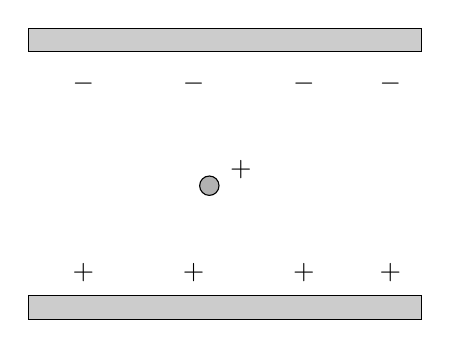
\begin{tikzpicture}
  % top plate (negative)
  \fill[gray!40] (0,3.4) rectangle (5,3.7);
  \draw (0,3.4) rectangle (5,3.7);
  \node at (0.7,3.0) {$-$};
  \node at (2.1,3.0) {$-$};
  \node at (3.5,3.0) {$-$};
  \node at (4.6,3.0) {$-$};
  % positive test charge
  \filldraw[fill=gray!60] (2.3,1.7) circle (3.5pt);
  \node at (2.7,1.9) {$+$};
  % bottom plate (positive)
  \fill[gray!40] (0,0) rectangle (5,0.3);
  \draw (0,0) rectangle (5,0.3);
  \node at (0.7,0.6) {$+$};
  \node at (2.1,0.6) {$+$};
  \node at (3.5,0.6) {$+$};
  \node at (4.6,0.6) {$+$};
\end{tikzpicture}
